\documentclass[9pt,a4paper]{extarticle}
\usepackage[utf8]{inputenc}
\usepackage[T1]{fontenc}
\usepackage[brazil]{babel}
\usepackage{geometry}
\geometry{margin=2cm}
\usepackage{parskip}
\usepackage{amsmath, amssymb}
\usepackage{xcolor}
\usepackage{graphicx}
\usepackage{booktabs}
\usepackage{enumitem}
\usepackage{hyperref}
\usepackage{tikz}
\usetikzlibrary{positioning}

%\setlist{nosep}

\title{Lista de Exercícios -- Busca em Espaço de Estados}
\author{BCC740 -- Inteligência Artificial \\ Prof. Rodrigo Silva}
\date{}

\begin{document}

\maketitle

\section*{Leitura Recomendada}
\begin{itemize}
  \item Capítulo 3 (\textit{Problem Solving as Search}) do livro \textbf{Poole \& Mackworth, Artificial Intelligence: Foundations of Computational Agents (3e)}, disponível em \url{https://artint.info/}.
\end{itemize}

% ==============================================================
\section{Questões Teóricas}
% ==============================================================

\begin{enumerate}

  \item (Cap. 1) O que é um \textbf{agente}? Explique como ele interage com o ambiente.
  \item (Cap. 1) Quando dizemos que um agente é \textbf{inteligente}? Quais propriedades o caracterizam como tal?
  
  \item (Seção 3.1) O que significa \textbf{busca} no contexto dos métodos de resolução de problemas apresentados no livro?
  \item (Seção 3.2) Quais são as \textbf{premissas} de um problema de busca em espaços de estados?
  \item (Seção 3.2) Quais são os \textbf{componentes} formais de um problema de busca em espaços de estados?
  \item (Seção 3.3) Qual a relação entre \textbf{espaços de estados} e \textbf{grafos}?
  \item (Seção 3.3.1) Quais são os \textbf{componentes e objetivos} de um problema de busca em grafo?
  \item (Seção 3.4) Apresente o \textbf{algoritmo genérico de busca} e descreva suas principais estruturas de dados.
  \item (Seção 3.5.1) Mostre um exemplo de execução do \textbf{algoritmo de busca em profundidade (DFS)}. Apresente o estado da fronteira a cada iteração.
  \item (Seção 3.5.2) Mostre um exemplo de execução do \textbf{algoritmo de busca em largura (BFS)}. Apresente o estado da fronteira a cada iteração.
  \item (Seção 3.5) Apresente uma discussão sobre os custo de\textbf{tempo e espaço} dos algoritmos \textbf{DFS} e \textbf{BFS}. 

  \item Considere o problema de encontrar um caminho no labirinto abaixo. O objetivo é ir da posição \textbf{s} até a posição \textbf{g}. O agente pode se mover nas quatro direções (cima, baixo, esquerda, direita). 

  \begin{enumerate}[label*=\alph*)]
    \item Numere os nós expandidos (visitados) por um agente que implementa \textbf{busca em profundidade}. A ordem das ações é: cima, esquerda, direita e baixo. (Assuma poda de ciclos.)
    \item Numere os nós expandidos por um agente que implementa a \textbf{busca de menor custo primeiro}.
    \item Escreva em cada nó o valor da \textbf{heurística de distância de Manhattan} (distância em unidades horizontais + verticais até o objetivo).
    \item Numere os nós expandidos por um agente que implementa a \textbf{busca gulosa} utilizando a heurística acima. (Assuma poda de ciclos.)
    \item Numere os nós expandidos por um agente que implementa o algoritmo \textbf{$A^{\*}$}, considerando a distância de Manhattan como custo e heurística.

  \end{enumerate}

\end{enumerate}

    \begin{figure}[!ht]
      \centering
      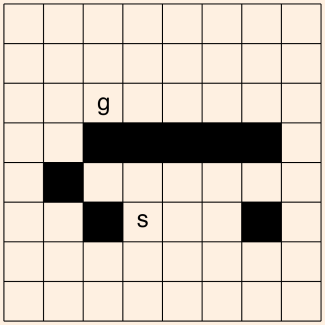
\includegraphics[width=0.35\textwidth]{grid.png}
    \end{figure}
    
    \begin{figure}[!ht]
      \centering
      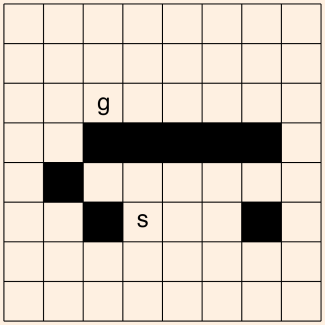
\includegraphics[width=0.35\textwidth]{grid.png}
    \end{figure}

        \begin{figure}[!ht]
      \centering
      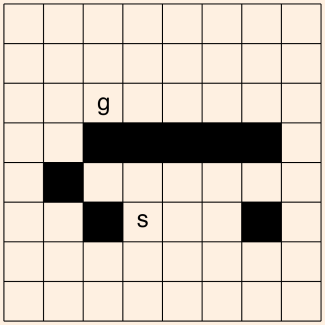
\includegraphics[width=0.35\textwidth]{grid.png}
    \end{figure}

        \begin{figure}[!ht]
      \centering
      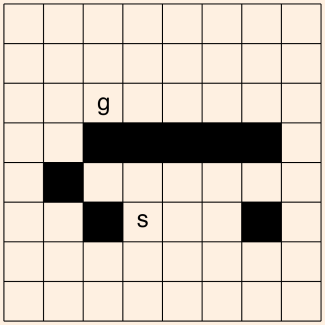
\includegraphics[width=0.35\textwidth]{grid.png}
    \end{figure}

        \begin{figure}[!ht]
      \centering
      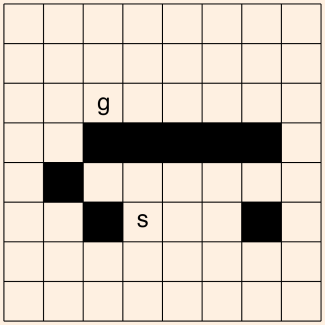
\includegraphics[width=0.35\textwidth]{grid.png}
    \end{figure}

\pagebreak
% ==============================================================
\section{Trabalho Prático -- Missionários e Canibais}
% ==============================================================

Neste trabalho, o estudante deverá implementar um agente que resolva o \textbf{problema dos missionários e canibais}, conforme discutido em aula.

\subsection*{Descrição do Problema}

Três missionários e três canibais estão em uma margem do rio e precisam atravessar usando um barco que comporta no máximo duas pessoas.  
Em nenhum momento pode haver mais canibais do que missionários em uma margem (exceto quando não houver missionários nela).  

O problema deve ser resolvido como um \textbf{problema de busca}, utilizando as representações:
\[
(M_E, C_E, B)
\]
onde $M_E$ é o número de missionários à esquerda, $C_E$ é o número de canibais à esquerda, e $B \in \{E, D\}$ indica a posição do barco.

\subsection*{O que deve ser implementado}

\begin{enumerate}
  \item Crie uma classe \texttt{MissionariesAndCannibals}, com:
  \begin{itemize}
    \item Representação do estado inicial e estado meta;
    \item Método \texttt{successors(state)} que gera todos os estados válidos (sem violar as restrições);
    \item Método \texttt{is\_goal(state)} que testa se o estado é uma solução;
    \item Custo unitário por travessia.
  \end{itemize}
  
  \item Implemente versões de \textbf{BFS}, \textbf{DFS} e \textbf{UCS} (utilizando o algoritmo genérico de busca apresentado em aula).
  
  \item Mostre a sequência de ações e o número de nós expandidos para cada método.
\end{enumerate}

\subsection*{Variações}

Explore versões modificadas do problema e observe como o espaço de estados muda:
\begin{itemize}
  \item Mude a \textbf{capacidade do barco} (ex.: 3 lugares);
  \item Altere o número de missionários e canibais (ex.: 4 de cada lado);
  \item Atribua \textbf{custos diferentes} para certas travessias (ex.: atravessar com dois canibais custa mais);
  \item Adicione \textbf{restrições assimétricas} (ex.: o barco deve sempre retornar com alguém);
  \item Faça comparações entre o desempenho dos algoritmos para cada variação.
\end{itemize}

\subsection*{Entrega}

\begin{itemize}
  \item \texttt{missionaries.py} com a implementação do problema;
  \item \texttt{agents.py} com as funções de busca adaptadas;
  \item Um arquivo \texttt{main.py} que execute os testes e exiba a sequência de ações e o número de nós expandidos.
\end{itemize}

\end{document}
